\documentclass{article}
\usepackage[utf8]{inputenc}

\title{Chem-131C-Lec21}

\author{swflynn}
\date{May 2017}

\usepackage{natbib}
\usepackage{graphicx}
\usepackage{braket}
\usepackage{amsmath}
\usepackage[margin=0.7in]{geometry}
\usepackage{subfigure}
\usepackage{url}
\usepackage{float}
\usepackage[version=3]{mhchem}

\begin{document}

\maketitle

\section*{Lecture 21; 5/24/17}
The beauty of thermodynamics comes from the small number of assumptions needed to completely describe the topic.
The famous Thermodynamics book by Callen makes 4 claims at the beginning of the text, and the remainder of the subject is derived. 

\subsection*{Gibbs Again}
We are now going to look at Chapter 26 in McQuarrie, Chemical Reactions. 
Now that we are introducing other chemical species into our analysis we will need to incorporate these chemical species into our fundamental equations. 
Consider G(T,P,N), we can construct a total differential as follows
\begin{equation}
\begin{split}
dG &= \left(\frac{\partial G}{\partial T}\right)_{P,N}dT +  \left(\frac{\partial G}{\partial P}\right)_{N,T}dP + \left(\frac{\partial G}{\partial N}\right)_{T,P}dN \\
dG &= -SdT + VdP + \mu dN
\end{split}
\end{equation}
As we investigated earlier, we can use the fundamental equations to define thermodynamic variables as various partial derivatives.

If we consider a constant N and T process we can simplify our total differential to get the Gibbs Free Energy as a function of Pressure. 
\begin{equation}
\begin{split}
    dG &= \left(\frac{\partial G}{\partial P}\right)_{N,T}dP\\
    dG &= VdP\\
    \Delta G &= nRT \ln \left(\frac{P_f}{P_i}\right)
    \end{split}
\end{equation}
Note when we assume an ideal gas, we are simply assuming a linear dependence between variables in our equation of state, this linear approximation is what generates all of the natural logarithm dependencies. 

\subsection*{Chemical Reactions}
Consider one of the simplest chemical reactions.
\begin{equation}\begin{split}
    A &\rightleftharpoons B \\
    n_A &\quad n_B
    \end{split}
\end{equation}
In this chemical system we have conservation of mass, all of the A we react turns into B and the reciprocal direction. 
Another way to say this, A and B are linked through the stoichometry of the reaction, they are not independent. 
So this means we really only need one variable to track the 'extent' of the reaction. 
\begin{equation}
    n = n_A + n_B = \text{constant} \implies |dn_B| = |dn_A|
\end{equation}
In this picture we would now need to define G as G(T, P, n$_A$, n$_B$). 
Again we can write down the total differential, which will contain all 4 parameters now, if we assume a constant T and P we can simplify to two terms. 
\begin{equation}
\begin{split}
dG &= \left(\frac{\partial G}{\partial T}\right)_{P,n}dT +  \left(\frac{\partial G}{\partial P}\right)_{n,T}dP + \left(\frac{\partial G}{\partial n_A}\right)_{T,P,n_B}dn_A + \left(\frac{\partial G}{\partial n_B}\right)_{T,P,n_A}dn_B \\
\xrightarrow{\Delta(T,P)=0}&= \left(\frac{\partial G}{\partial n_A}\right)_{T,P,n_B}dn_A + \left(\frac{\partial G}{\partial n_B}\right)_{T,P,n_A}dn_B \\
dG &= \mu_Adn_A + \mu_B dn_B
\end{split}
\end{equation}
Where we define a chemical potential for each species of interest. 
As we noted above the two variables here are not independent, we can define a new variable, called the \textbf{Extent of Reaction} ($\xi$). 
For this simple two component system we define the following. 
\begin{equation}
dn_B = d\xi \qquad dn_A = -d\xi
\end{equation}
Here our sign convention says the $\xi$ increases as we generate B (this choice is arbitrary). 
With this definition we can now simplify our dG equation. 
\begin{equation}
\begin{split}
    dG &= \mu_Adn_A + \mu_B dn_B \\
    &= -\mu_Ad\xi + \mu_B d\xi = (\mu_B - \mu_A)d\xi \\
    dG &= \Delta_rGd\xi
\end{split}
\end{equation}
Where we have made another definition, the Gibbs energy of reaction 
\begin{equation}
\Delta_rG \equiv \left(\frac{\partial G}{\partial \xi}\right)_{T,P}
\end{equation}

Let's now consider a plot of G vs $\xi$, based on our reaction components we will have a function with one critical point/inflection point, and the slope will be $\Delta_rG$.
\begin{figure}[! h]
    \centering
    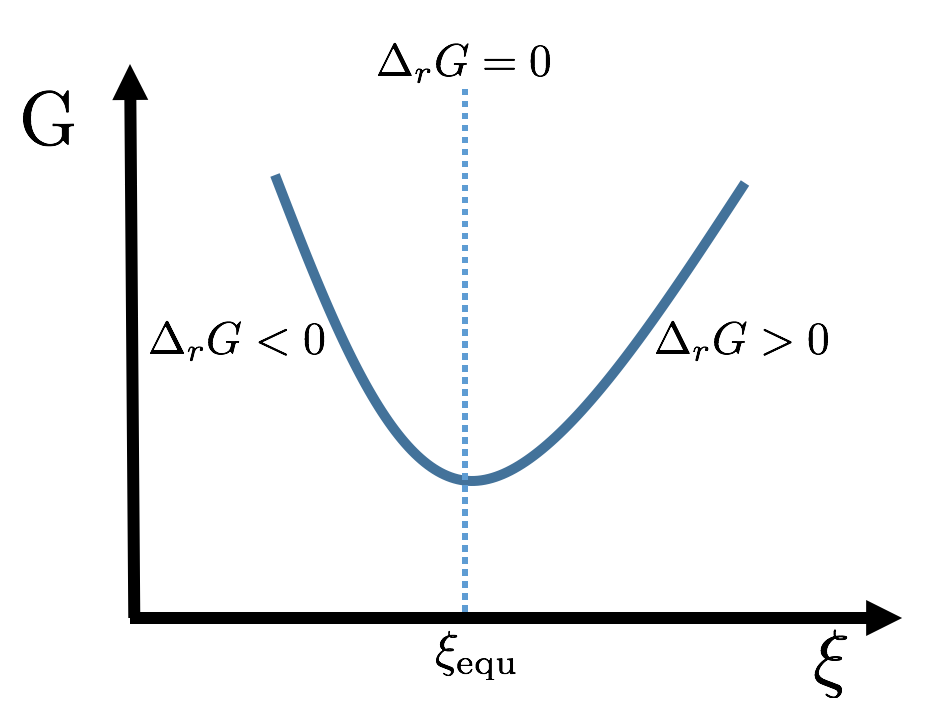
\includegraphics[width=7cm]{rxnG.png}
    \caption{Gibbs and $\xi$. The slope of the curve represents the Gibbs Energy of Reaction. One minimum $\exists$ at $\mu_A = \mu_B$ }
    \label{fig:rxnG}
\end{figure}
At the equilibrium we have a slope of 0. 
\begin{equation}
\mu_B - \mu_A = \Delta_rG = 0 \implies \mu_A = \mu_B
\end{equation}
\begin{center}
  \begin{tabular}{ | l | c | r |}
    \hline
    $\Delta_rG < 0$ & $\mu_A > \mu_B$ & Spontaneous A $\rightarrow$ B \\ \hline
     $\Delta_rG > 0$ & $\mu_A < \mu_B$ & Spontaneous A $\leftarrow$ B \\ \hline
     $\Delta_rG = 0$ & $\mu_A = \mu_B$ & Equilibrium \\
    \hline
  \end{tabular}
\end{center}

\subsection*{Ideal Gas Equilibrium}
For this simple model we see that the change in Gibbs is simply due to the change in composition; $\Delta_rG = \mu_B - \mu_A$.
\begin{equation}
\mu_A = \mu_A^0 + RT \ln\left(\frac{P_A}{P_A^0}\right) \qquad \mu_B = \mu_B^0 + RT \ln\left(\frac{P_B}{P_B^0}\right)
\end{equation}
Here the $^0$ is referring to an arbitrary reference state. 
If we substitute these equations in to our definition for the $\Delta _rG$ we can write. 
\begin{equation}
\begin{split}
    \Delta_rG &= \mu_B - \mu_A = \mu_B^0 + RT \ln\left(\frac{P_B}{P_B^0}\right) - \mu_A^0 - RT \ln\left(\frac{P_A}{P_A^0}\right) \\
    &= \mu_B^0 - \mu_A^0 + RT\ln\left(\frac{P_B P_A^0}{P_B^0 P_A}\right) \xrightarrow{P_A^0 = P_B^0 \equiv P^0} \\
    \Delta_rG &= \mu_B^0 - \mu_A^0 + RT\ln\left(\frac{P_B }{P_A}\right) \\
    \Delta_rG &= \mu_B^0 - \mu_A^0 + RT\ln\left(Q\right)
\end{split}
\end{equation}
Here the last line is yet another term we are defining called the \textbf{Reaction Quotient} (not the partition function or heat). 
\begin{equation}
Q \equiv \frac{P_B}{P_A}
\end{equation}

\end{document}